\subsection{המטען האפקטיבי}
ב\autoref{fig:He_effective_charge} ניתן לראות כי המטען האפקטיבי שאלקטרון רואה עבור מרחק גדול מהראשית, הוא $-1$, כלומר הכל חוץ ממנו. עבור מרחק קרוב לראשית הוא בקושי רואה את האלקטרון השני ואפקטיבית הוא מרגיש בעיקר את הגרעים, אז המטען קרוב ל־$-2$.

\begin{figure}[h!]
    \centering
    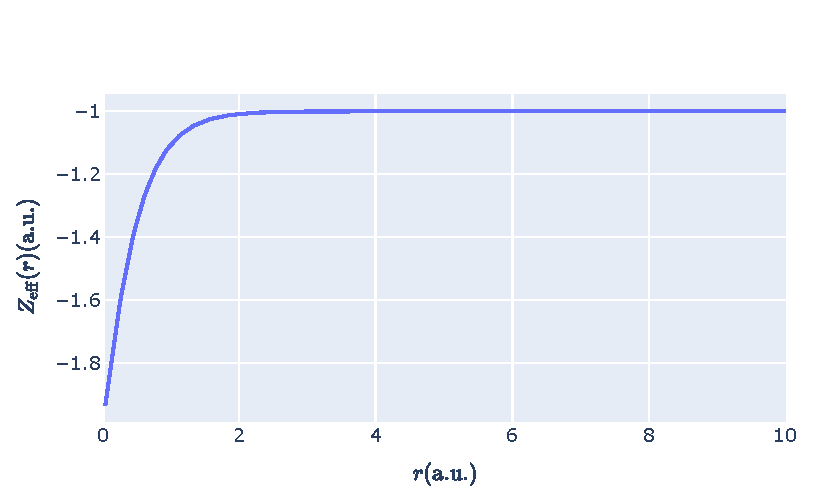
\includegraphics[width=0.5\linewidth]{plots/helium_atom/effective_charge.eps}
    \caption{המטען האפקטיבי באיטרציה האחרונה}
    \label{fig:He_effective_charge}
\end{figure}
% ניתן לראות כי המטען האפקטיבי שאלקטרון רואה עבור מרחק גדול מהראשית, הוא $-1$, כלומר הכל חוץ ממנו. עבור מרחק קרוב לראשית הוא בקושי רואה את האלקטרון השני ואפקטיבית הוא מרגיש בעיקר את הגרעים, אז המטען קרוב ל־$-2$.
